% Distillation Pipeline — Single Source → Structured Distillate
% Compile with: pdflatex distillation-pipeline.tex
\documentclass[border=14pt]{standalone}

\usepackage[T1]{fontenc}
\usepackage[english]{babel}
\usepackage{lmodern}
\usepackage{amsmath}
\usepackage{xcolor}
\usepackage{tikz}
\usetikzlibrary{
    decorations.pathmorphing,
    decorations.pathreplacing,
    arrows.meta,
    positioning,
    calc,
    shapes.geometric,
    shapes.symbols,
    backgrounds,
    fit
}

%% ---------- Colour palette ----------
\definecolor{ink}        {HTML}{1F2433}
\definecolor{soft}       {HTML}{9CA3AF}
\definecolor{nodebg}     {HTML}{F4F6FA}
\definecolor{accent}     {HTML}{3A6E5B}  % distillate / key flow
\definecolor{lens}       {HTML}{C8553D}

%% --- 6 dimension colours (one per lens) ---
\definecolor{c1}{HTML}{4A6FA5}\definecolor{c1bg}{HTML}{EBF1F9}  % Topic
\definecolor{c2}{HTML}{C9883A}\definecolor{c2bg}{HTML}{FBF2DD}  % Author
\definecolor{c3}{HTML}{B85C92}\definecolor{c3bg}{HTML}{F8E8F0}  % Implicit
\definecolor{c4}{HTML}{4F8A6B}\definecolor{c4bg}{HTML}{E7F0EA}  % Theories
\definecolor{c5}{HTML}{C8553D}\definecolor{c5bg}{HTML}{FBEBE6}  % Conclusions
\definecolor{c6}{HTML}{5B6E8C}\definecolor{c6bg}{HTML}{ECEFF4}  % Methodology

\definecolor{stagebg}    {HTML}{FBFCFE}
\definecolor{stageborder}{HTML}{C8CFDB}

\begin{document}
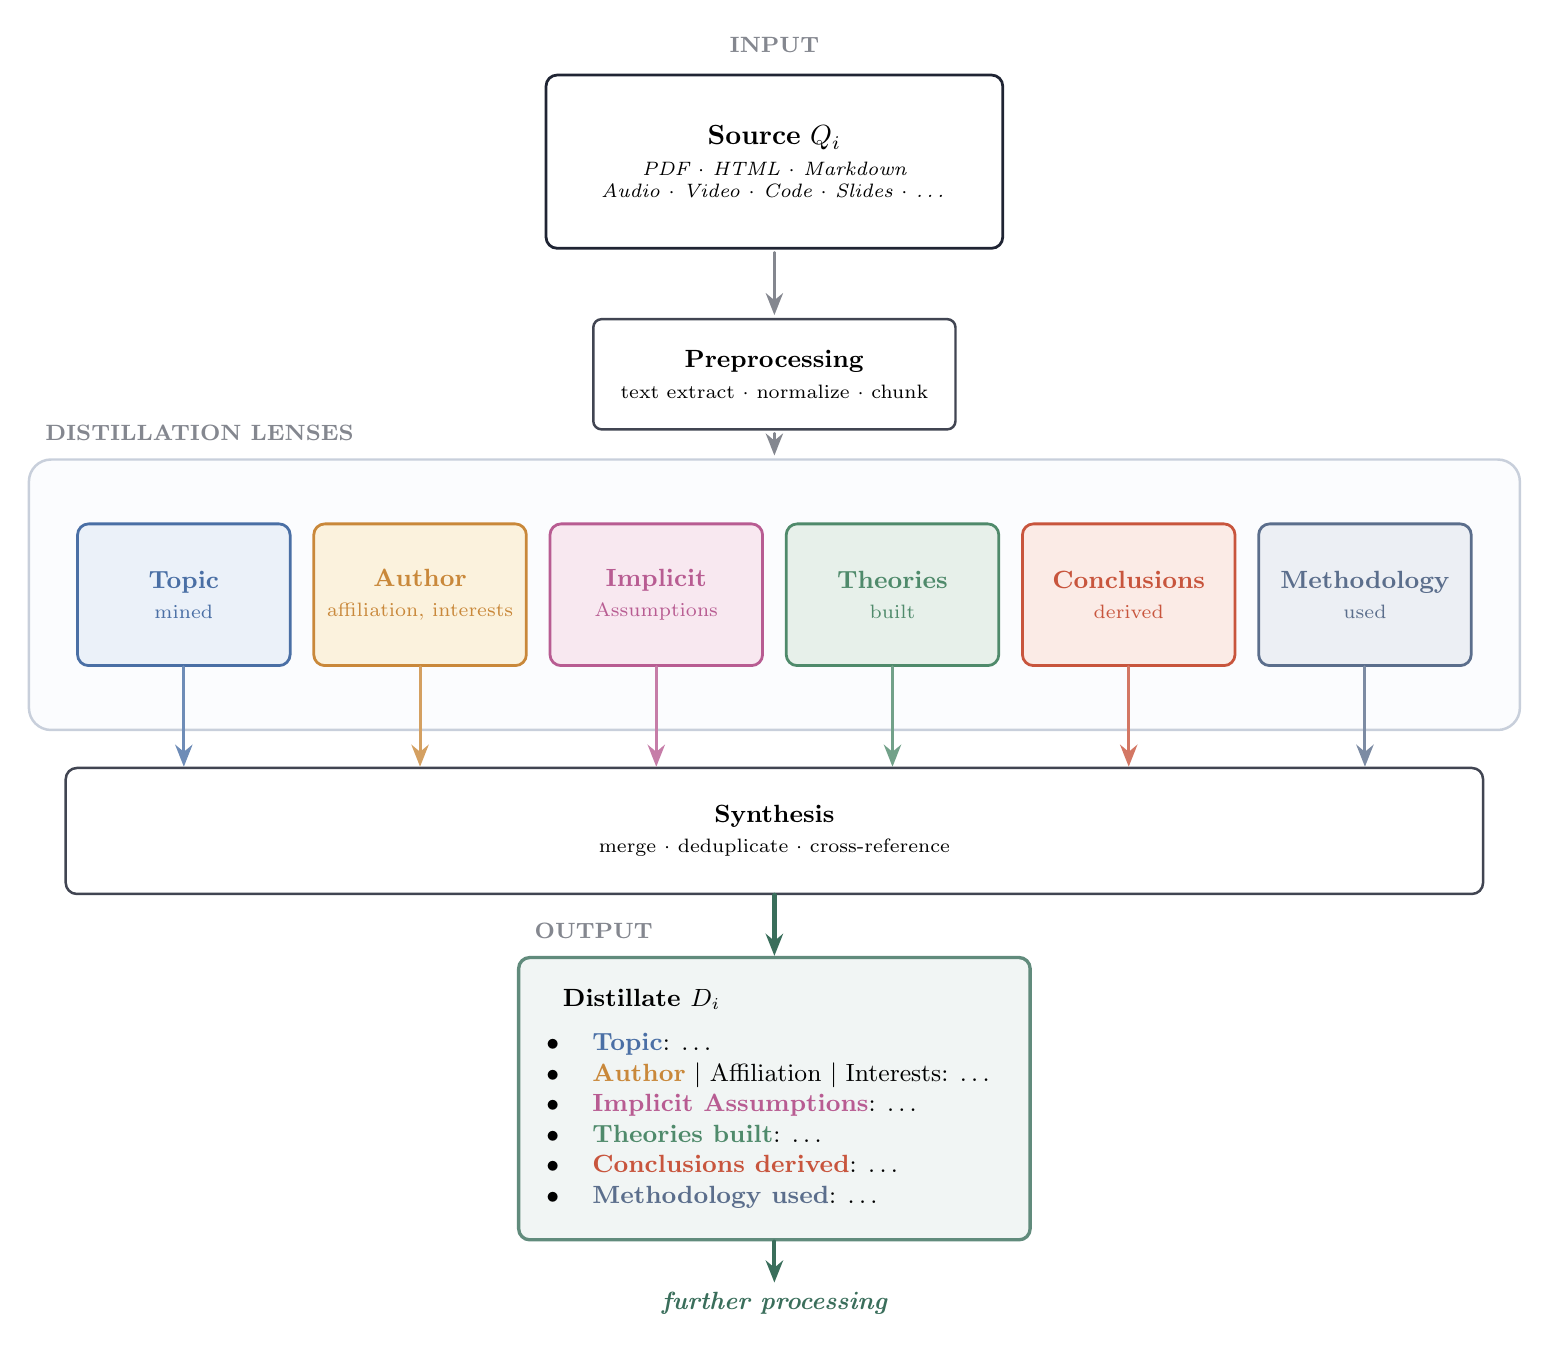
\begin{tikzpicture}[
    line cap=round, line join=round,
    >={Stealth[length=2.8mm, width=2.2mm]},
    %% --- semantic styles ---
    outline/.style       = {draw=ink, line width=0.8pt},
    sourcebox/.style     = {rectangle, draw=ink, fill=white, line width=1pt,
                            rounded corners=4pt, minimum width=58mm,
                            minimum height=22mm, font=\normalsize,
                            align=center},
    procbox/.style       = {rectangle, draw=ink!85, fill=white, line width=0.9pt,
                            rounded corners=3pt, minimum width=46mm,
                            minimum height=14mm, font=\small,
                            align=center, inner sep=4pt},
    synbar/.style        = {rectangle, draw=ink!85, fill=white, line width=0.9pt,
                            rounded corners=4pt, minimum width=180mm,
                            minimum height=16mm, font=\small,
                            align=center, inner sep=4pt},
    lensbox/.style       = {rectangle, line width=1pt, rounded corners=4pt,
                            minimum width=27mm, minimum height=18mm,
                            font=\small\bfseries, align=center, inner sep=3pt},
    distbox/.style       = {rectangle, draw=accent!80, fill=accent!7,
                            line width=1.2pt, rounded corners=4pt,
                            inner sep=10pt, font=\small, align=left},
    keyflow/.style       = {->, draw=accent, line width=1.8pt},
    procflow/.style      = {->, draw=ink!55, line width=1pt,
                            shorten >=1pt, shorten <=1pt},
    sectionlabel/.style  = {font=\footnotesize\bfseries, text=ink!55}
]

%% =====================================================
%% INPUT — Source with format examples
%% =====================================================
\node[sourcebox] (SRC) at (0, 5.5) {%
    \textbf{Source} $Q_i$\\[3pt]
    \begin{minipage}{50mm}\centering
        \scriptsize\itshape
        PDF $\cdot$ HTML $\cdot$ Markdown\\
        Audio $\cdot$ Video $\cdot$ Code $\cdot$ Slides $\cdot$ \ldots
    \end{minipage}
};
\node[sectionlabel, anchor=south] at ($(SRC.north) + (0, 1.5mm)$) {INPUT};

%% =====================================================
%% Preprocessing
%% =====================================================
\node[procbox] (PRE) at (0, 2.8) {%
    \textbf{Preprocessing}\\
    \scriptsize text extract $\cdot$ normalize $\cdot$ chunk
};
\draw[procflow] (SRC) -- (PRE);

%% =====================================================
%% DISTILLATION LENSES — 6 dimensions in a SINGLE ROW
%% =====================================================
\node[lensbox, fill=c1bg, draw=c1, text=c1] (L1) at (-7.5, 0)
    {Topic\\\scriptsize\normalfont mined};
\node[lensbox, fill=c2bg, draw=c2, text=c2] (L2) at (-4.5, 0)
    {Author\\\scriptsize\normalfont affiliation, interests};
\node[lensbox, fill=c3bg, draw=c3, text=c3] (L3) at (-1.5, 0)
    {Implicit\\\scriptsize\normalfont Assumptions};
\node[lensbox, fill=c4bg, draw=c4, text=c4] (L4) at ( 1.5, 0)
    {Theories\\\scriptsize\normalfont built};
\node[lensbox, fill=c5bg, draw=c5, text=c5] (L5) at ( 4.5, 0)
    {Conclusions\\\scriptsize\normalfont derived};
\node[lensbox, fill=c6bg, draw=c6, text=c6] (L6) at ( 7.5, 0)
    {Methodology\\\scriptsize\normalfont used};

% Container around lenses
\begin{scope}[on background layer]
    \node[draw=stageborder, fill=stagebg, rounded corners=8pt,
          line width=0.9pt,
          inner xsep=6mm, inner ysep=8mm,
          fit=(L1) (L6)] (LBOX) {};
\end{scope}
\node[sectionlabel, anchor=south west]
    at ($(LBOX.north west) + (1mm, 1mm)$) {DISTILLATION LENSES};

% Single fan-out from PRE into the lens container
\draw[procflow] (PRE.south) -- (LBOX.north);

%% =====================================================
%% SYNTHESIS — wide bar so every lens drops STRAIGHT down
%% =====================================================
\node[synbar] (SYN) at (0, -3.0) {%
    \textbf{Synthesis}\\
    \scriptsize merge $\cdot$ deduplicate $\cdot$ cross-reference
};

% Six straight vertical colour-coded arrows — no overlap, no curves
\foreach \L/\C in {L1/c1, L2/c2, L3/c3, L4/c4, L5/c5, L6/c6}
    \draw[->, draw=\C!80, line width=1.1pt]
        (\L.south) -- (\L.south |- SYN.north);

%% =====================================================
%% OUTPUT — Distillate as a structured record
%% =====================================================
\node[distbox] (DIST) at (0, -6.4) {%
    \begin{tabular}{@{}rl@{}}
        \multicolumn{2}{l}{\bfseries Distillate $D_i$}\\[5pt]
        $\bullet$ & {\color{c1}\bfseries Topic}: \ldots\\
        $\bullet$ & {\color{c2}\bfseries Author} $\mid$ Affiliation $\mid$ Interests: \ldots\\
        $\bullet$ & {\color{c3}\bfseries Implicit Assumptions}: \ldots\\
        $\bullet$ & {\color{c4}\bfseries Theories built}: \ldots\\
        $\bullet$ & {\color{c5}\bfseries Conclusions derived}: \ldots\\
        $\bullet$ & {\color{c6}\bfseries Methodology used}: \ldots\\
    \end{tabular}
};

\draw[keyflow] (SYN) -- (DIST);
\node[sectionlabel, anchor=south west]
    at ($(DIST.north west) + (1mm, 1mm)$) {OUTPUT};

%% =====================================================
%% Further processing
%% =====================================================
\node[font=\small\bfseries\itshape, text=accent] (FP) at (0, -9.0)
    {further processing};
\draw[keyflow, line width=1.4pt] (DIST.south) -- (FP);

\end{tikzpicture}
\end{document}
